\subsection{GitHubの使い方}
解析ソースコードの共有および測定データの共有にGitHubを使うことを推奨する.
必要な情報のほとんどウェブ検索によって得られる(\href{https://tech-blog.rakus.co.jp/entry/20200529/git}{例}). 
このうち簡単な説明を以下で示す.

\subsubsection{git, GitHubとは}
gitはコマンドライン上でテキストファイル群のバージョン(変更履歴)管理を行うためのツールである.

gitはバージョン管理を図\ref{fig:git_desc}のように行っており, 各開発者の持つローカルリポジトリと共有のためのリモートリポジトリが存在する\cite{github}.
リポジトリとはバージョン管理の対象となるファイル群のことを指す。
gitでは、ファイルの状態を好きな時に更新履歴として保存しておくことができる。一度変更したファイルを過去の状態に戻したり、変更差分を表示したりできる。
変更のながれを分岐して記録しているのがブランチである。他のブランチの影響を受けず、また、変更をmergeすることもできる。

gitで複数人での開発を行う流れは簡単に、
\begin{enumerate}
\item 開発者がリモートリポジトリから最新のソースコードをローカルリポジトリにコピーする(clone, fetch, pull)
\item ローカルリポジトリで開発する
\item コミットしたい変更ファイルをステージングする(add)
\item 変更をローカルリポジトリに保存する(commit)
\item 変更をリモートリポジトリに反映する(push)
\end{enumerate}
ここで, リモートリポジトリをホストするサービスとしてGitHubがある(GitHub以外にもある).
\begin{figure}[h]
    \centering
    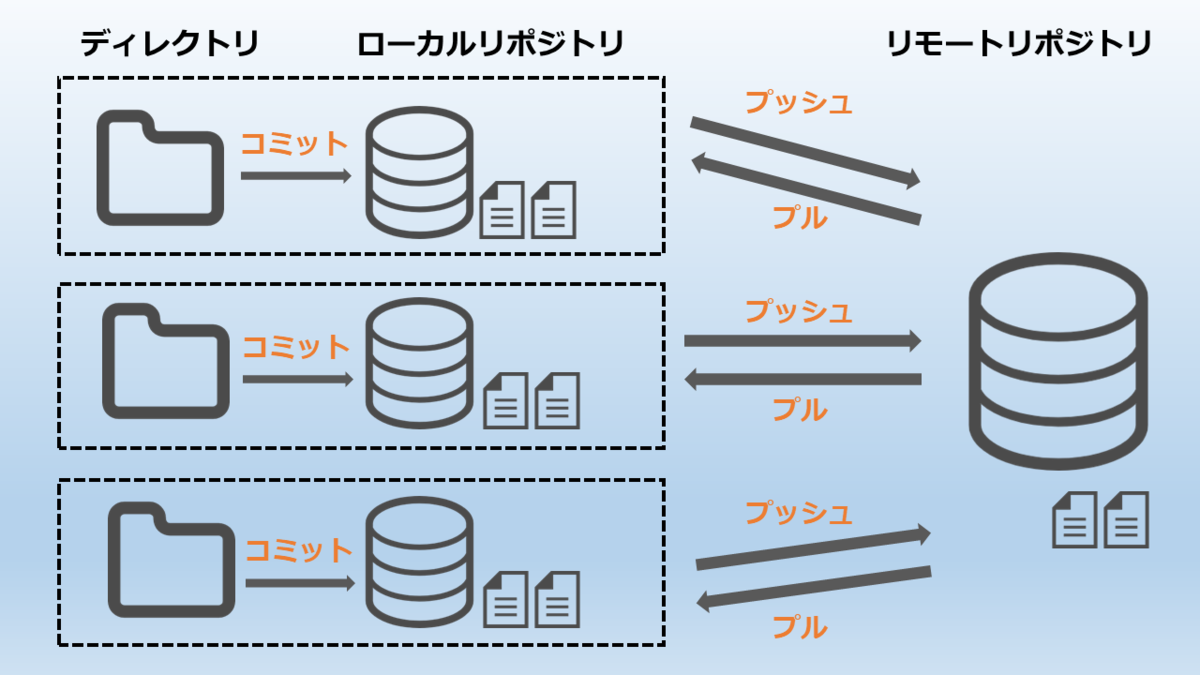
\includegraphics[height=4cm]{../git_desc.png}
    \caption{gitの概念図\cite{github}}
    \label{fig:git_desc}
\end{figure}

\subsubsection{gitの簡単な使い方}
\begin{itemize}
    \item リモートリポジトリをローカルマシンにダウンロード(クローン)する
    \begin{lstlisting}
$ git clone (address)
    \end{lstlisting}
    \item ローカルにあるブランチの一覧を見る
    \begin{lstlisting}
$ git branch
    \end{lstlisting}
    \item ブランチを作る
    \begin{lstlisting}
$ git branch new_branch
    \end{lstlisting}
    \item 別のブランチに移る
    \begin{lstlisting}
$ git chackout new_branch
    \end{lstlisting}
    \item ローカルリポジトリの変更状況を表示する
    \begin{lstlisting}
$ git status
    \end{lstlisting}
    \item 変更をアップする
    \begin{lstlisting}
$ git add modified_file01
$ git add modified_file02
$ git commit -m "commit message"
$ git push origin new_branch
    \end{lstlisting}
    \item メインブランチの変更を現在のブランチに落としてくる
    \begin{lstlisting}
$ git pull origin main
    \end{lstlisting}
\end{itemize}

